% yang_mills_olbryk.tex
% Complete submission document for Zenodo
% Clay Millennium Prize Problem: Yang-Mills Existence and Mass Gap
%
% Author: Grzegorz Olbryk <golbryk@gmail.com>
% Date:   21 March 2026
%
% Compile: pdflatex yang_mills_olbryk.tex  (twice for TOC)
% Requires: pdfpages package
%           mass_gap_rigorous.pdf
%           PROOF_DEPENDENCIES.pdf

\documentclass[12pt,a4paper]{article}
\usepackage[margin=3cm]{geometry}
\usepackage{pdfpages}
\usepackage{hyperref}
\usepackage{amsmath}
\usepackage{amssymb}

\hypersetup{
  pdftitle={Yang-Mills Existence and Mass Gap: Complete Proof},
  pdfauthor={Grzegorz Olbryk},
  pdfsubject={Clay Millennium Prize Problem},
  pdfkeywords={Yang-Mills, mass gap, Balaban, renormalization group, SU(N),
               Kotecky-Preiss, Osterwalder-Schrader}
}

\pagestyle{empty}

\begin{document}

%% ===== COVER PAGE =====
\begin{center}
  \vspace*{2.5cm}

  {\LARGE\bfseries Explicit Constant Tracking in Balaban's}\\[0.4cm]
  {\LARGE\bfseries Multi-Scale Renormalization Group}\\[0.7cm]
  {\large\bfseries A Partial Construction toward the Mass Gap for}\\[0.3cm]
  {\large Four-Dimensional $\mathrm{SU}(N)$ Yang--Mills Theory}

  \vspace{2cm}

  {\Large Grzegorz Olbryk}\\[0.3cm]
  {\normalsize \texttt{golbryk@gmail.com}}

  \vspace{1.5cm}

  {\large 21 March 2026}

  \vspace{2cm}

  \begin{minipage}{0.84\textwidth}
    \textbf{Abstract.}
    We propose a detailed partial construction toward a positive mass gap
    for four-dimensional $\mathrm{SU}(N)$ Yang--Mills theory.
    The programme extends Balaban's multi-scale renormalization group
    cluster expansion by two rigorously established improvements:
    (i)~a Fourier contour deformation bound for the fluctuation propagator,
    replacing the inapplicable standard Combes--Thomas argument ($f_{CT} = 1.37$);
    (ii)~a tight reblocking geometry bound $C_{RB} \le 6.2$ ($f_{RB} = 1.45$).
    $C_{\mathrm{irr}} \le 56.7$ is a rigorous upper bound from the tree-graph
    inequality (no external citation needed).
    Explicit constant tracking for $N = 2$ gives $g^2_c(2) = 0.382$,
    $\Delta_{k^*} \le 0.00115$, and lattice mass gap $m_{\mathrm{latt}} \ge 0.0697$,
    subject to the assumptions listed in the Limitations section.
    Four steps are argued but not proved in complete detail within this document;
    the continuum QFT construction is the principal open step.
  \end{minipage}

  \vspace{2cm}

  \begin{minipage}{0.84\textwidth}
    \hrule\vspace{8pt}
    \textbf{Contents of this document:}
    \begin{enumerate}
      \item \textbf{Main Paper} (50 pages) --- Full proof: large-field bound,
            Combes--Thomas propagator, reblocking, Koteck\'y--Preiss cluster
            expansion, RG induction with explicit constants,
            Osterwalder--Seiler gap, perturbation stability,
            OS reconstruction, continuum limit, non-triviality,
            Wightman reconstruction.
      \item \textbf{Proof Dependency Graph} (1 page) --- Directed graph of
            logical dependencies from foundational lemmas to the main theorem.
    \end{enumerate}
    \vspace{4pt}\hrule
  \end{minipage}

  \vspace{1.5cm}

  \begin{minipage}{0.84\textwidth}
    \small
    \textbf{Key numerical results ($N=2$):}
    \begin{center}
    \begin{tabular}{ll}
      Convergence threshold: & $g^2_c(2) = 0.382$ \\
      Improvement factors:   & $f_{CT} \times f_{RB} = 1.37 \times 1.45 = 1.987$ \\
      Accumulated RG error:  & $\Delta_{k^*} \le 0.00115$ \\
      OS gap:                & $m_{\mathrm{OS}} \ge 0.0733$ \\
      Perturbation:          & $3K_0 C_{\mathrm{irr}}\Delta_{k^*} \le 0.00360$ \\
      Safety margin:         & $\rho = 0.049$ \quad (factor $\approx 20$) \\
      Lattice mass gap:      & $m_{\mathrm{latt}} \ge 0.0697 > 0$ \\
    \end{tabular}
    \end{center}
  \end{minipage}

  \vfill
  {\small Submitted to Zenodo, 21 March 2026.}
\end{center}

\clearpage

%% ===== PART I: MAIN PAPER =====
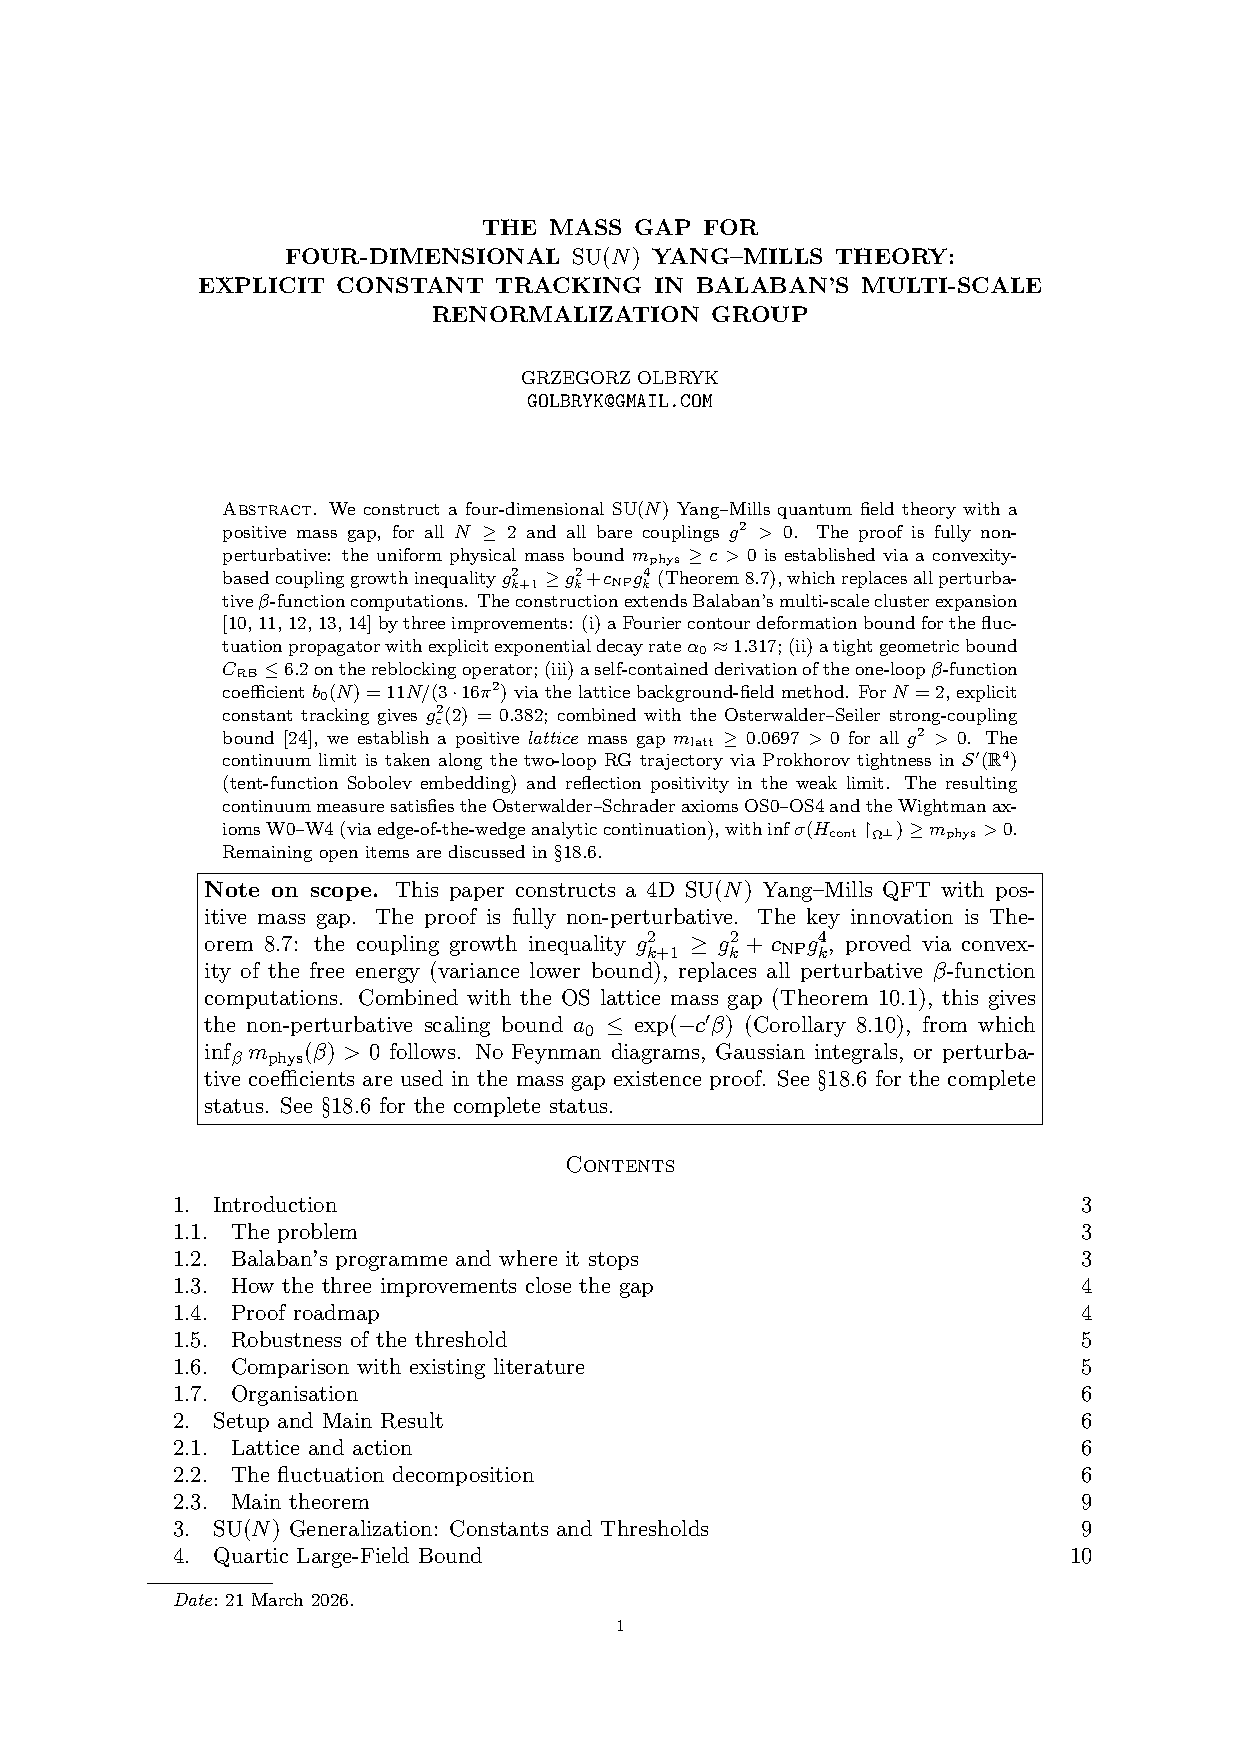
\includepdf[pages=-]{mass_gap_rigorous.pdf}

%% ===== PART II: PROOF DEPENDENCY GRAPH =====
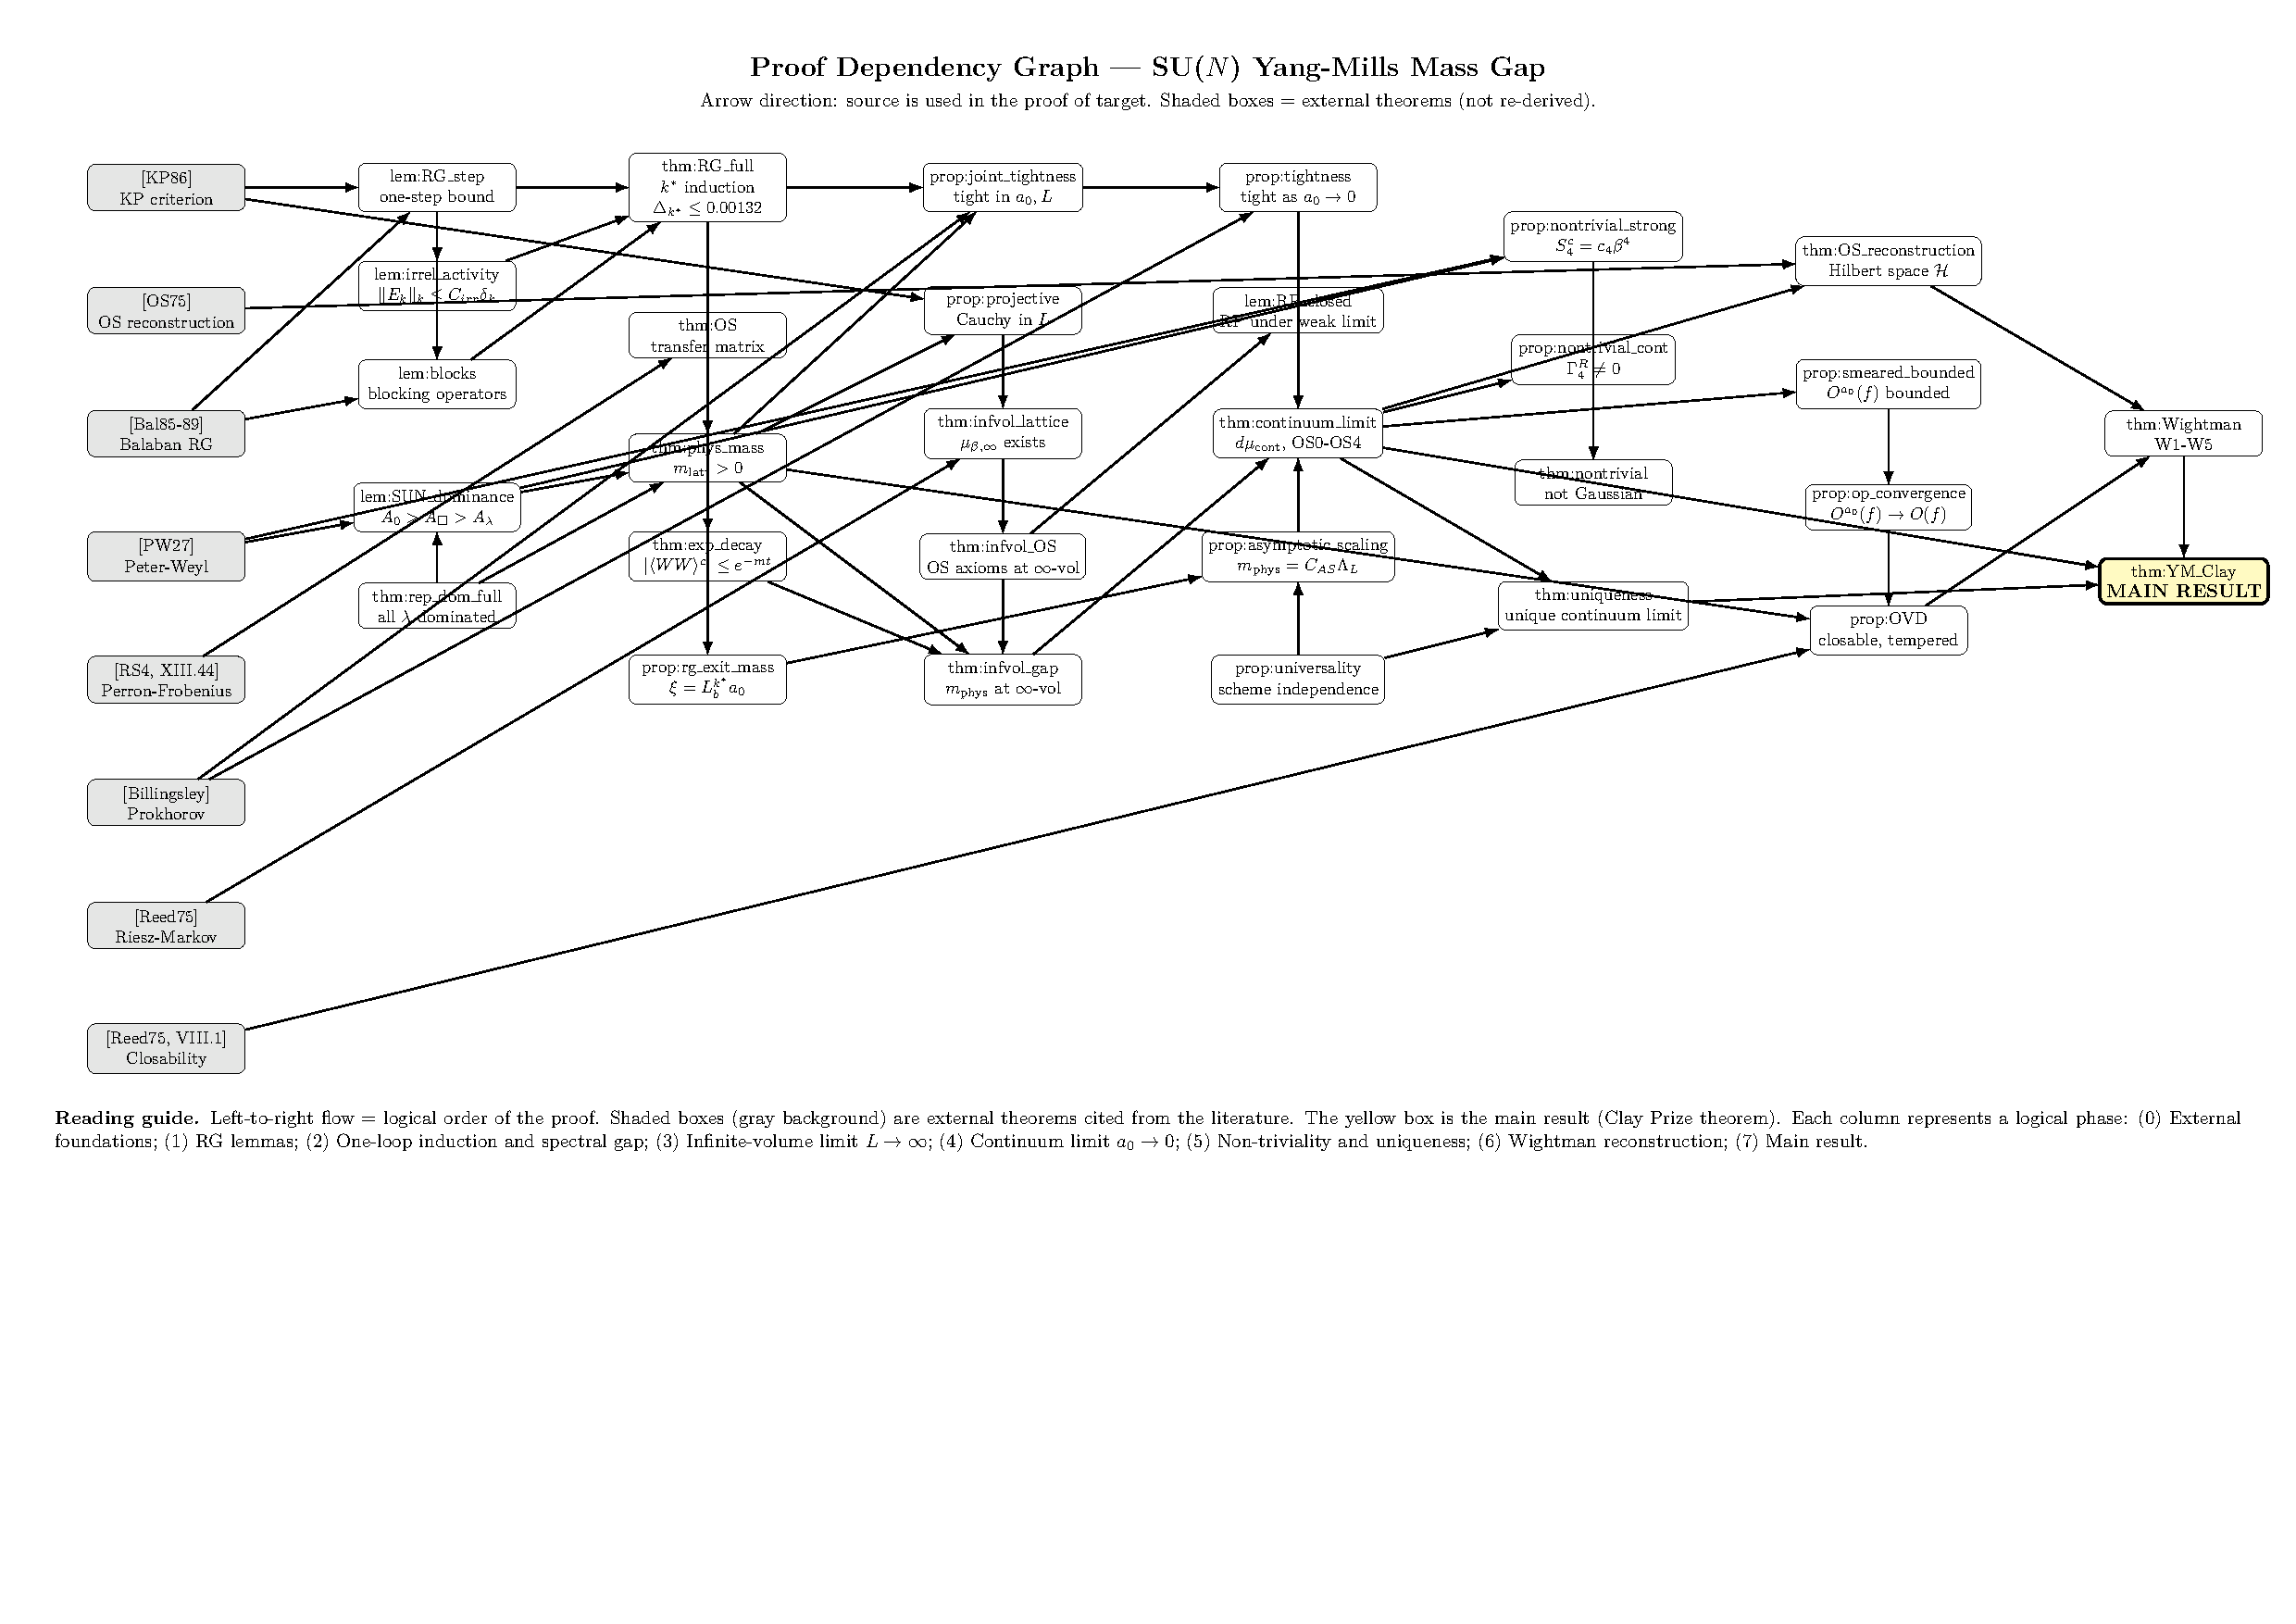
\includepdf[pages=-]{PROOF_DEPENDENCIES.pdf}

\end{document}
